\documentclass[a4paper,11pt]{exam}
%\printanswers % pour imprimer les réponses (corrigé)
\noprintanswers % Pour ne pas imprimer les réponses (énoncé)
\addpoints % Pour compter les points
% \noaddpoints % pour ne pas compter les points
%\qformat{\textbf{\thequestion ) } }
%\qformat{\textbf{\thequestion )}} % Pour définir le style des questions (facultatif)
\usepackage{color} % définit une nouvelle couleur
\shadedsolutions % définit le style des réponses
% \framedsolutions % définit le style des réponses
\definecolor{SolutionColor}{rgb}{0.8,0.9,1} % bleu ciel
\renewcommand{\solutiontitle}{\noindent\textbf{Solution:}\par\noindent} % Définit le titre des solutions




\makeatletter

\def\maketitle{{\centering%
	\par{\huge\textbf{\@title}}%
	\par{\@date}%
	\par}}


\renewcommand{\thesubsection}{\Alph{subsection}.}   

\makeatother

\lhead{NOM Pr\'enom :}
\rhead{\textbf{Les r\'eponses doivent \^etre justifi\'ees et r\'edig\'ees}}
\cfoot{\thepage / \pageref{LastPage}}


%\usepackage{../../pas-math}
%\usepackage{../../moncours}


%\usepackage{pas-cours}
%-------------------------------------------------------------------------------
%          -Packages nécessaires pour écrire en Français et en UTF8-
%-------------------------------------------------------------------------------
\usepackage[utf8]{inputenc}
\usepackage[frenchb]{babel}
%\usepackage{numprint}
\usepackage[T1]{fontenc}
%\usepackage{lmodern}
\usepackage{textcomp}
\usepackage[french, boxed]{algorithm2e}
\usepackage{hyperref}


%-------------------------------------------------------------------------------

%-------------------------------------------------------------------------------
%                          -Outils de mise en forme-
%-------------------------------------------------------------------------------
\usepackage{hyperref}
\hypersetup{pdfstartview=XYZ}
%\usepackage{enumerate}
\usepackage{graphicx}
\usepackage{multicol}
\usepackage{tabularx}
\usepackage{multirow}
\usepackage{color}
\usepackage{eurosym}


\usepackage{anysize} %%pour pouvoir mettre les marges qu'on veut
%\marginsize{2.5cm}{2.5cm}{2.5cm}{2.5cm}

\usepackage{indentfirst} %%pour que les premier paragraphes soient aussi indentés
\usepackage{verbatim}
\usepackage{enumitem}
\usepackage{booktabs}
\usepackage[usenames,dvipsnames,svgnames,table]{xcolor}

\usepackage{variations}

%-------------------------------------------------------------------------------


%-------------------------------------------------------------------------------
%                  -Nécessaires pour écrire des mathématiques-
%-------------------------------------------------------------------------------
\usepackage{amsfonts}
\usepackage{amssymb}
\usepackage{amsmath}
\usepackage{amsthm}
\usepackage{tikz}
\usepackage{xlop}
\usepackage[output-decimal-marker={,}]{siunitx}
%-------------------------------------------------------------------------------

%-------------------------------------------------------------------------------
%                  -Nécessaires pour écrire des formules chimiquess-
%-------------------------------------------------------------------------------

\usepackage[version=4]{mhchem}

%-------------------------------------------------------------------------------
% Pour pouvoir exploiter les fichiers directement dans beamer
\newcommand{\pause}{\ }
%-------------------------------------------------------------------------------
%                    - Mise en forme avancée
%-------------------------------------------------------------------------------

\usepackage{ifthen}
\usepackage{ifmtarg}


\newcommand{\ifTrue}[2]{\ifthenelse{\equal{#1}{true}}{#2}{$\qquad \qquad$}}

%\newcommand{\kword}[1]{\textcolor{red}{\underline{#1}}}
%-------------------------------------------------------------------------------

%-------------------------------------------------------------------------------
%                     -Mise en forme d'exercices-
%-------------------------------------------------------------------------------
%\newtheoremstyle{exostyle}
%{\topsep}% espace avant
%{\topsep}% espace apres
%{}% Police utilisee par le style de thm
%{}% Indentation (vide = aucune, \parindent = indentation paragraphe)
%{\bfseries}% Police du titre de thm
%{.}% Signe de ponctuation apres le titre du thm
%{ }% Espace apres le titre du thm (\newline = linebreak)
%{\thmname{#1}\thmnumber{ #2}\thmnote{. \normalfont{\textit{#3}}}}% composants du titre du thm : \thmname = nom du thm, \thmnumber = numéro du thm, \thmnote = sous-titre du thm

%\theoremstyle{exostyle}
%\newtheorem{exercice}{Exercice}
%
%\newenvironment{questions}{
%\begin{enumerate}[\hspace{12pt}\bfseries\itshape a.]}{\end{enumerate}
%} %mettre un 1 à la place du a si on veut des numéros au lieu de lettres pour les questions 
%-------------------------------------------------------------------------------

%-------------------------------------------------------------------------------
%                    - Mise en forme de tableaux -
%-------------------------------------------------------------------------------

\renewcommand{\arraystretch}{1.7}

\setlength{\tabcolsep}{1.2cm}

%-------------------------------------------------------------------------------



%-------------------------------------------------------------------------------
%                    - Racourcis d'écriture -
%-------------------------------------------------------------------------------
%Droites
\newcommand{\dte}[1]{$(#1)$}
\newcommand{\fig}[1]{figure $#1$}
\newcommand{\sym}{symétrique}
\newcommand{\syms}{symétriques}
\newcommand{\asym}{axe de symétrie}
\newcommand{\asyms}{axes de symétrie}
\newcommand{\seg}[1]{$[#1]$}
\newcommand{\monAngle}[1]{$\widehat{#1}$}
\newcommand{\bissec}{bissectrice}
\newcommand{\mediat}{médiatrice}
\newcommand{\ddte}[1]{$[#1)$}


% Angles orientés (couples de vecteurs)
\newcommand{\aopp}[2]{(\vec{#1}, \vec{#2})} %Les deuc vecteurs sont positifs
\newcommand{\aopn}[2]{(\vec{#1}, -\vec{#2})} %Le second vecteur est négatif
\newcommand{\aonp}[2]{(-\vec{#1}, \vec{#2})} %Le premier vecteur est négatif
\newcommand{\aonn}[2]{(-\vec{#1}, -\vec{#2})} %Les deux vecteurs sont négatifs

%Ensembles mathématiques
\newcommand{\naturels}{\mathbb{N}} %Nombres naturels
\newcommand{\relatifs}{\mathbb{Z}} %Nombres relatifs
\newcommand{\rationnels}{\mathbb{Q}} %Nombres rationnels
\newcommand{\reels}{\mathbb{R}} %Nombres réels
\newcommand{\complexes}{\mathbb{C}} %Nombres complexes


%Intégration des parenthèses aux cosinus
\newcommand{\cosP}[1]{\cos\left(#1\right)}
\newcommand{\sinP}[1]{\sin\left(#1\right)}


%Probas stats
\newcommand{\stat}{statistique}
\newcommand{\stats}{statistiques}


\newcommand{\homo}{homothétie}
\newcommand{\homos}{homothéties}


\newcommand{\mycoord}[3]{(\textcolor{red}{\num{#1}} ; \textcolor{Green}{\num{#2}} ; \textcolor{blue}{\num{#3}})}
%-------------------------------------------------------------------------------

%-------------------------------------------------------------------------------
%                    - Mise en page -
%-------------------------------------------------------------------------------

\newcommand{\twoCol}[1]{\begin{multicols}{2}#1\end{multicols}}


\setenumerate[1]{font=\bfseries,label=\textit{\alph*})}
\setenumerate[2]{font=\bfseries,label=\arabic*)}


%-------------------------------------------------------------------------------
%                    - Elements cours -
%-------------------------------------------------------------------------------

%Correction d'exercice
\newcommand{\exoSec}[2]{\subsection*{Exercice #1 page #2}}
%-------------------------------------------------------------------------------
%                    - raccourcis d'écriture -
%-------------------------------------------------------------------------------

%Mise en évidence de termes clés
\newcommand{\mykw}[1]{\textcolor{red}{\underline{\textbf{#1}}}}

%Exercices
\newcommand{\exo}[2]{exercice #1 page #2}
\newcommand{\Exo}[2]{Exercice #1 page #2}

\renewcommand{\pause}{\ }

%Intervalles
\newcommand{\interOO}[2]{$]$#1 , #2$[$}
\newcommand{\interOF}[2]{$]$#1 , #2$]$}
\newcommand{\interFO}[2]{$[$#1 , #2$[$}
\newcommand{\interFF}[2]{$[$#1 , #2$]$}



%\usepackage{fullpage}
\author{\ }
\date{20 Mai 2019}
\title{Devoir Maison de Sciences Physiques}


\begin{document}
%	\usepackage{fancyhdr}
%	
%	\pagestyle{fancy}
%	\fancyhf{}
	%\rhead{Share\LaTeX}

	\maketitle
%	
%\begin{small}
%	\begin{center}
%		\begin{tabular}{|@{\ }l@{}|@{\ }c@{\ }|}
%			\hline
%			\textbf{Compétence} & \textbf{Maitrise} \\
%			\hline
%		Exploiter les lois de l’électricité. \ \ &  \ \ \ \\
%			\hline
%			%Conservation de la masse lors d’une transformation chimique. &  \\
%			%\hline			
%			Relation tension-courant : loi d’Ohm. \ &  \\
%			\hline
%		\end{tabular}
%	\end{center}
%\end{small}	
	
	
%\vspace*{-0.5cm}	

%Seul l'\ref{ex:structure} est à faire sur le sujet. Le soin et la qualité de rédaction sont pris en compte dans la notation.


%\section{\'Equations de réaction}

Ajuster les équations de réactions suivantes :
\begin{questions}
	\question $CH_4 + ....O_2 \rightarrow ....CO_2 + ....H_2O$
	
	\question $C_7H_{16} + ....O_2 \rightarrow ....CO_2 + ....H_2O$	
	
	\question $C_6H_{2}O + ....O_2 \rightarrow ....CO_2 + ....H_2O$
\end{questions}

%
%\section{À chaque modèle sa formule}
\begin{questions}
	\question \'A partir de ces dessins de modèles, donner la formule des molécules suivantes.

	\begin{center}
		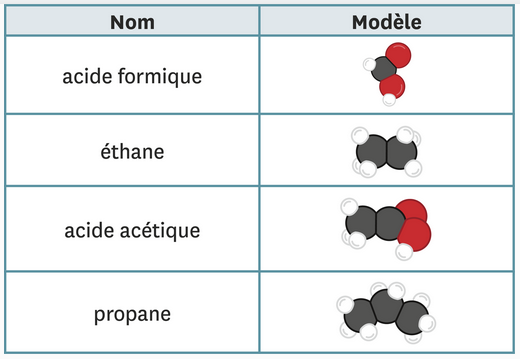
\includegraphics[scale=0.6]{img/exemples}
	\end{center}
	\fillwithdottedlines{2cm}
	
\end{questions}

%\section{Composition des molécules}


\begin{questions}
	\question Donner la composition des molécules suivantes :
	
	\begin{parts}
		\part l'éthylène $C_2H_4$	
		\fillwithdottedlines{1cm}
		
		\part le monoxyde d'azote $NO$	
		\fillwithdottedlines{1cm}
		
		\part l'ozone $O_3$	
		\fillwithdottedlines{1cm}	
		
		\part l'eau oxygénée $H_2O_2$	
		\fillwithdottedlines{1cm}
	\end{parts}

\end{questions}


%\newpage





%\section{Phrases à compléter (3 points)}

Recopier et compléter les phrases suivantes :

\begin{questions}
	\question[\half] Dans un circuit, plus la résistance augmente, plus l'intensité du courant $....$ .
	\begin{solution}
		Dans un circuit, plus la résistance augmente, plus l'intensité du courant \textbf{diminue}.
	\end{solution}
	
	\question[1] La résistance électrique se mesure à l'aide d'un $....$ et s'exprime en $....$ .
	\begin{solution}
		La résistance électrique se mesure à l'aide d'un \textbf{ohmmètre} et s'exprime en \textbf{ohm} .
	\end{solution}
	
	\question[1\half] La tension aux bornes d'un conducteur ohmique est $....$ à l'intensité du courant qui le traverse : c'est la loi d'Ohm, que l'on traduit par la relation : $....$ = $R$ $\times$  $....$.
	
	\begin{solution}
		La tension aux bornes d'un conducteur ohmique est \textbf{proportionnelle} à l'intensité du courant qui le traverse : c'est la loi d'Ohm, que l'on traduit par la relation : $\mathbf{U}$ = $R$ $\times$  $\mathbf{I}$.
	\end{solution}
\end{questions}





\section{Identification de solutions}

Au laboratoire, Enzo a trouvé un flacon sans étiquette, qui contient une solution incolore. 

\begin{center}
	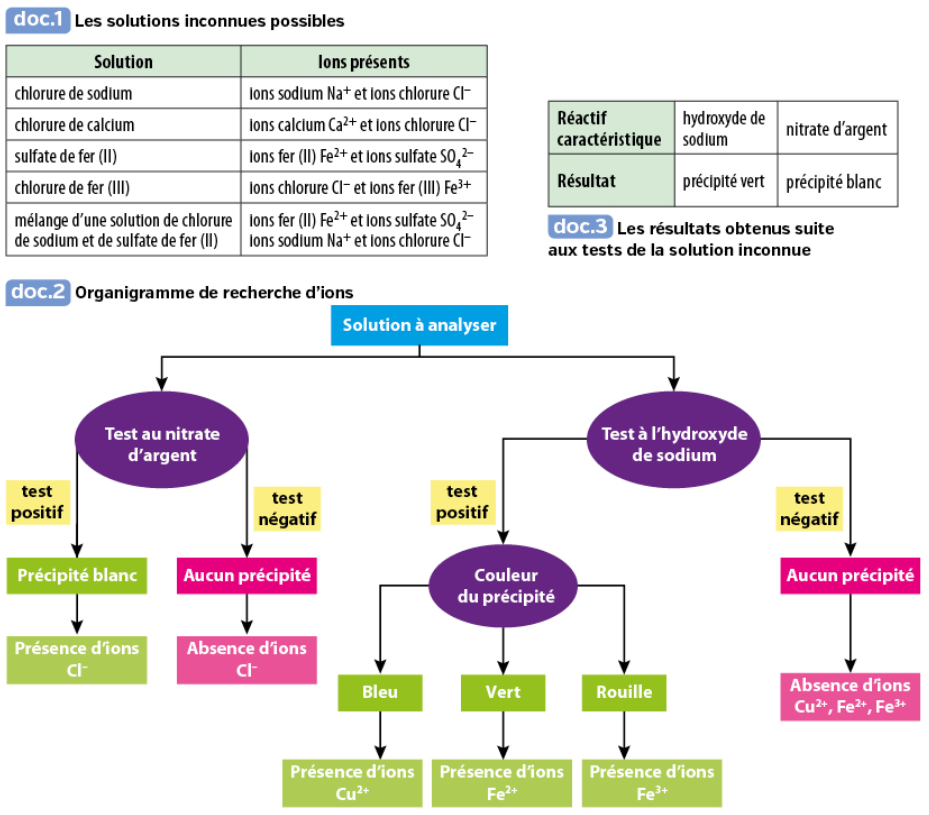
\includegraphics[scale=0.6]{img/docs}
\end{center}

\begin{questions}
	\question La solution inconnue est l'une de celles présentes dans le doc. 1. Quels tests doit-il faire pour l'identifier ? Décrire le protocole expérimental.
	\begin{solution}
		Pour identifier la solution inconnue, Enzo devra :
		\begin{itemize}
			\item verser quelques millilitres de la solution dans deux tubes à essais;
			\item ajouter quelques goutes de nitrate d'argent dans le premier tube;
			\item ajouter quelques goutes de soude dans le second tube;
			\item observer les résultats.
		\end{itemize}
	\end{solution}
	
	\question Représenter un de ces tests à l'aide d'un schéma.
	\begin{solution}
		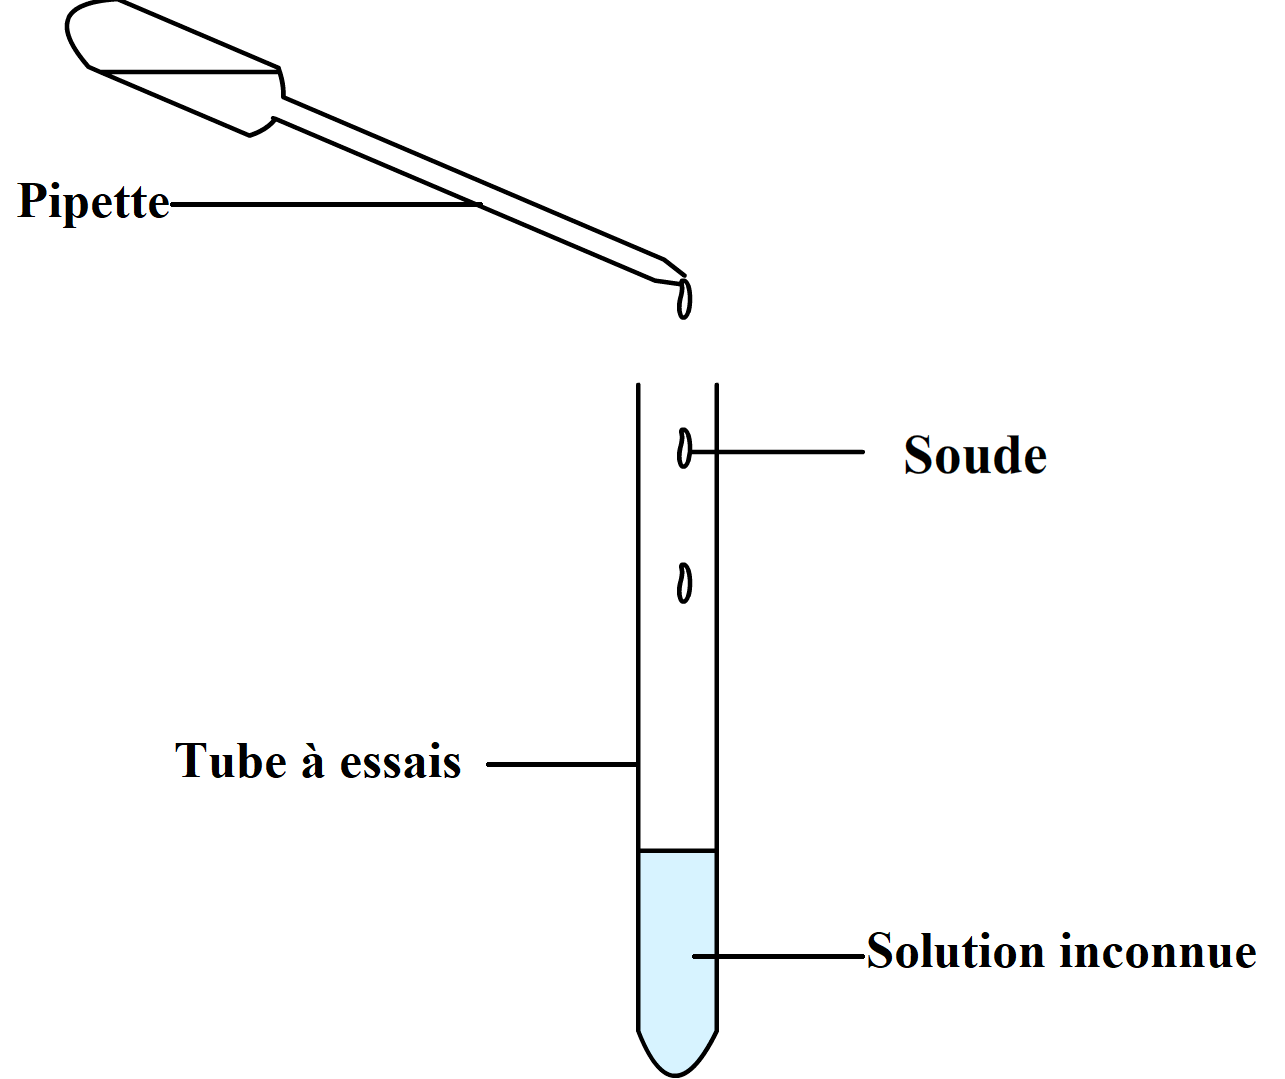
\includegraphics[scale=0.2]{img/ajout-soude}
	\end{solution}
	
	\question D'après les résultats obtenus présentés dans le doc. 3, quels ions ont été identifiés par les tests ? 
	\begin{solution}
		La solution à réagit avec la soude en formant un précipité vert et avec le nitrate d'argent en formant un précipité blanc. Elle contient donc des ions Fer II ($Fe^{2+}$)et Chlorure ($Cl^-$).
	\end{solution}
	
	\question Quelle est la solution contenue dans le flacon ?
	\begin{solution}
		La solution contenue dans le flacon est donc un mélange de chlorure de sodium et de sulfate de fer (II).
	\end{solution}
	
	\question Détailler la composition de chacun des ions présents dans la solution. (nombre de protons, nombre d'électrons, nombre de charges).
	\begin{solution}
		Cette solution contient des ions chlorure ($Cl^-$), sodium ($Na^+$), sulfate ($SO_4^{2-}$) et fer II ($Fe^{2+}$).
		\begin{itemize}
			\item Le numéro atomique de l'atome de chlore est 17, l'ion chlorure contient donc 17 protons, 18 électrons et 1 charge négative;
			
			\item Le numéro atomique de l'atome de sodium est 11, l'ion chlorure contient donc 11 protons, 10 électrons et 1 charge positive;
			
			\item L'ion sulfate est composé d'un atome de soufre et de 4 atomes d'oxygène. Le numéro atomique de l'atome de soufre est 16, celui de l'atome d'oxygène est 8. Donc l'ion sulfate compte 48 protons et 50 électrons, soit deux charges négatives. 
			
			\item Le numéro atomique de l'atome de fer est 26, l'ion fer II contient donc 26 protons, 24 électrons et 2 charges positives.
			
			.
		\end{itemize}
		
		
		
	\end{solution}
	
\end{questions}

\newpage

\section{Ions et santé}

On attribue plusieurs vertus au bicarbonates de sodium. On l'emploie notamment pour pour l'hygiène dentaire ou contre les maux d'estomac.

\begin{questions}
	\question L'ion Sodium est engendré par un atome de sodium lorsqu'il perd un électron.	
	\begin{parts}
		\part Combien de charges positives compte le noyau de l'ion sodium ?
		\begin{solution}
			L'ion sodium possède 17 protons dans son noyau donc 17 charges positives.
		\end{solution}
		
		\part Combien d'électrons composent cet ion ?
		\begin{solution}
			L'atome de sodium contient 17 électrons, donc l'ion sodium qui en a perdu un, en contient 16.
		\end{solution}
		
		\part \'Ecrire la formule chimique de cet ion.		
		\begin{solution}
			La formule chimique de l'ion sodium est $Na^+$.
		\end{solution}
	\end{parts}

	\question La formule chimique de l'ion bicarbonate s'écrit $HCO_3^-$
	\begin{parts}
		\part S'agit-il d'un cation ou d'un anion ?
		\begin{solution}
			L'ion bicarbonate est chargé négativement, c'est donc un anion.
		\end{solution}
	
		\part Combien d'atomes de chaque élément composent cet ion ?
		\begin{solution}
			Cet ion est composé d'un atome d'hydrogène, d'un de carbone et de 3 d'oxygène.
		\end{solution}
		
		\part Ce groupe d'atomes a perdu ou gagné un ou des électrons pour devenir un ion. Combien ?
		\begin{solution}
			C'est un anion donc il a gagné un électron.
		\end{solution}
	
	\end{parts}
\end{questions}


%\newpage 



%\newpage 
\section{Critique d'un protocole}

Pour vérifier la présence d'ions fer (III)  dans une solution, un élève propose le protocole sous la forme du schéma ci-dessous.


inserer schema  ex 19 p 24 bordas (espace)
\begin{questions}
	\question Rectifier l'erreur commise sur le réactif.
	
	\question Nommer le matériel utilisé.
	
	\question Quel matériel serait plus approprié ? Justifier.
\end{questions}

%\section{Caractéristiques d'un dipôle (3 points)}

Pierre a tracé le graphique caractéristique d'une résistance.

\begin{center}
	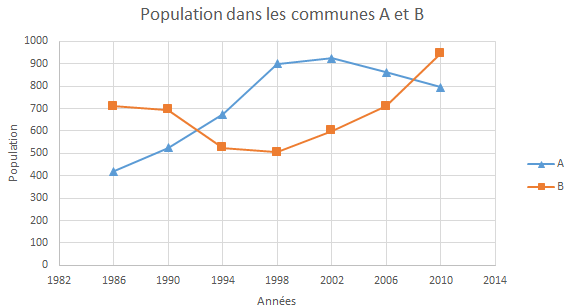
\includegraphics[scale=0.35]{img/graph}
\end{center}

\begin{questions}
	\question[1] Quelle est la tension aux bornes de la résistance lorsqu'elle est traversée par un courant d'intensité 60 $mA$ ?
	\begin{solution}
		Lorsqu'elle est traversée par un courant d'intensité 60 $mA$, la tension aux bornes de la résistance est 1 $V$.
	\end{solution}
	
	\question[1] Quelle est l'intensité du courant  dans la résistance si la tension à ses bornes est égale à 5 $V$ ?
	\begin{solution}
		Si la tension aux bornes de la résistance est égale à 5 $V$, elle est traversée par un courant de 300 $mA$.
	\end{solution}
	
	\question[1] Quelle est la valeur de cette résistance ?
	\begin{solution}
		D'après la loi d'Ohm, aux bornes de la résistance on a :
		
		\begin{eqnarray*}
			U &=& R \times I \\
			R &=& \frac{U}{I}\\
			R &=& \frac{1}{\num{0.3}}\\
			R &\approx& \num{3.33} \\
		\end{eqnarray*}
	
	Donc la valeur de cette résistance est \num{3.33} $\Omega$.
	\end{solution}
\end{questions}

%\section{Appareil à raclette (5 points)}

Lorsqu'elle est traversée par un courant électrique, une résistance produit de la chaleur, c'est l'effet Joule.
La résistance de l'appareil à raclette de Martin ne fonctionne plus ! Dans son garage, il trouve deux résistances qui pourraient peut-être convenir pour la remplacer. 
Les documents ci-dessous présentent le résultats de la mesure à l'ohmmètre des deux résistances et le descriptif technique de l'appareil à raclette.
%\begin{multicols}{2}
	\begin{center}
		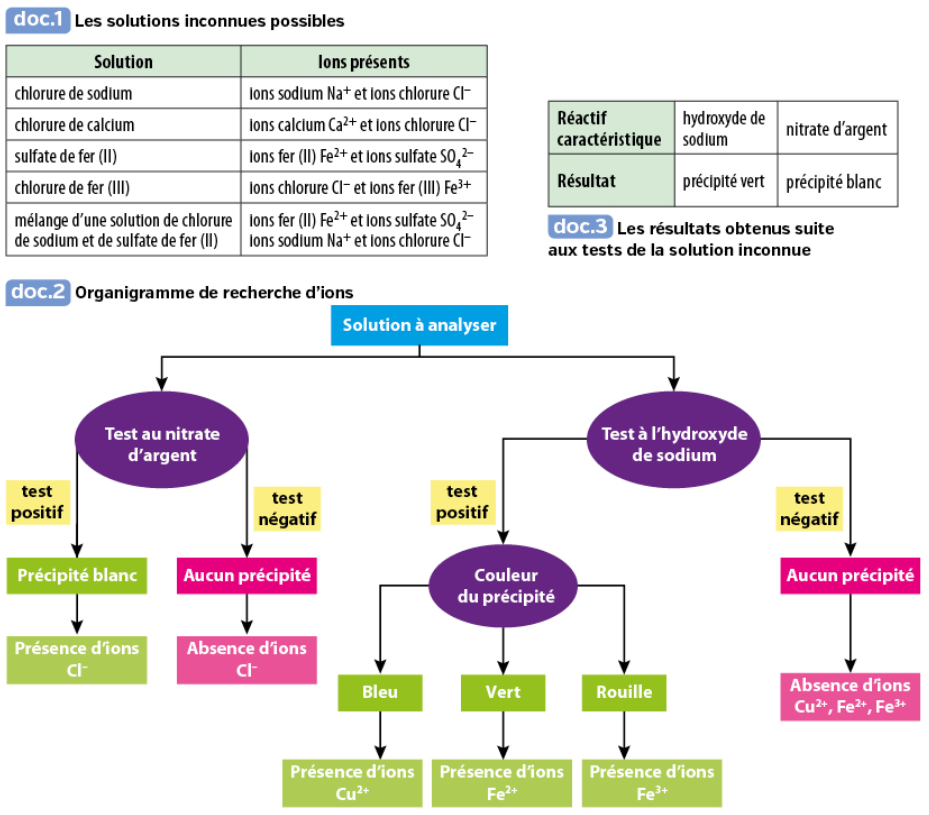
\includegraphics[scale=0.7]{img/docs}
		%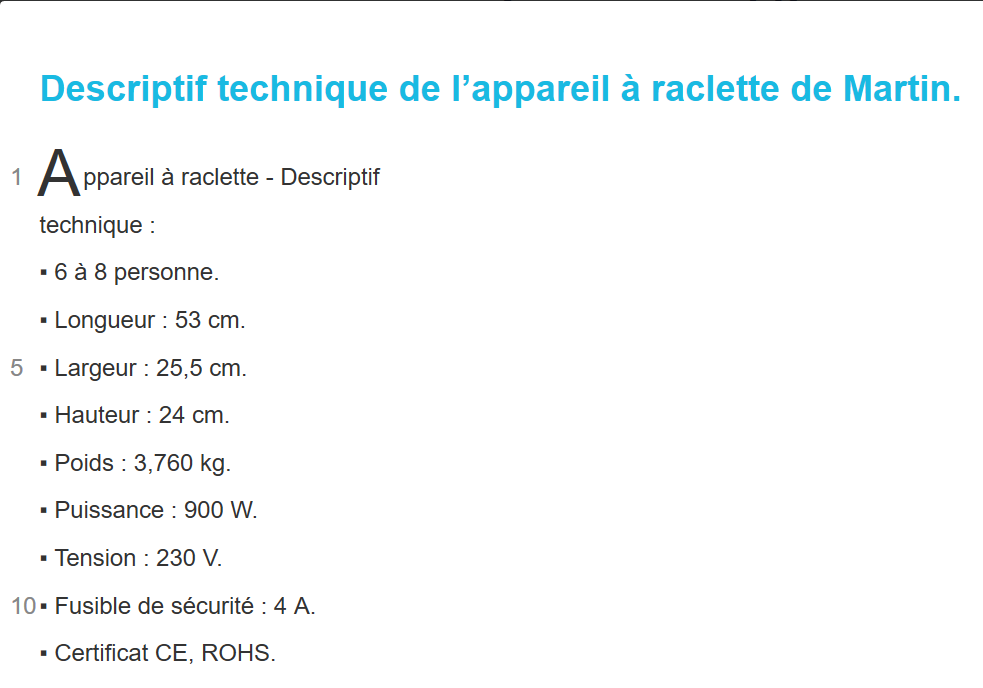
\includegraphics[scale=0.5]{img/doc2}
	\end{center}
%\end{multicols}

\begin{questions}
	\question[1] Quelles informations du descriptif technique permettront de savoir quelle sera la résistance appropriée ?
	\begin{solution}
		Sur le descriptif technique, le tension et nominale et la valeur du fusible permettront d'identifier la résistance appropriée.
	\end{solution}
	
	\question[1\half] Quelle valeur de résistance correspond à l'intensité maximale ?
	\begin{solution}
		L'intensité maximale supportée par l'appareil à raclette correspond à la valeur du fusible, c'est à dire 4 $A$. D'après la loi d'Ohm, on a :
		
		\begin{eqnarray*}
			U &=& R \times I \\
			R &=& \frac{U}{I} \\
			R &=& \frac{230}{4} \\
			R &=& \num{57.5}
		\end{eqnarray*}
	
	Donc l'intensité maximale correspond à une résistance de \num{57.5} $\Omega$.
	\end{solution}
	
	\question[1\half] Quelle résistance devra choisir Martin ?
	\begin{solution}
		Il devra choisir une valeur de résistance plus faible que la résistance maximale, c'est à dire la résistance B.
	\end{solution}
	
	\question[1] Que se passerait-il s'il choisissait l'autre ?
	\begin{solution}
		S'il choisissait l'autre, il dépasserait l'intensité maximale donc le fusible grillerait et ouvrirait le circuit pour éviter une surintensité.
	\end{solution}
\end{questions}




 
%\newpage
%
%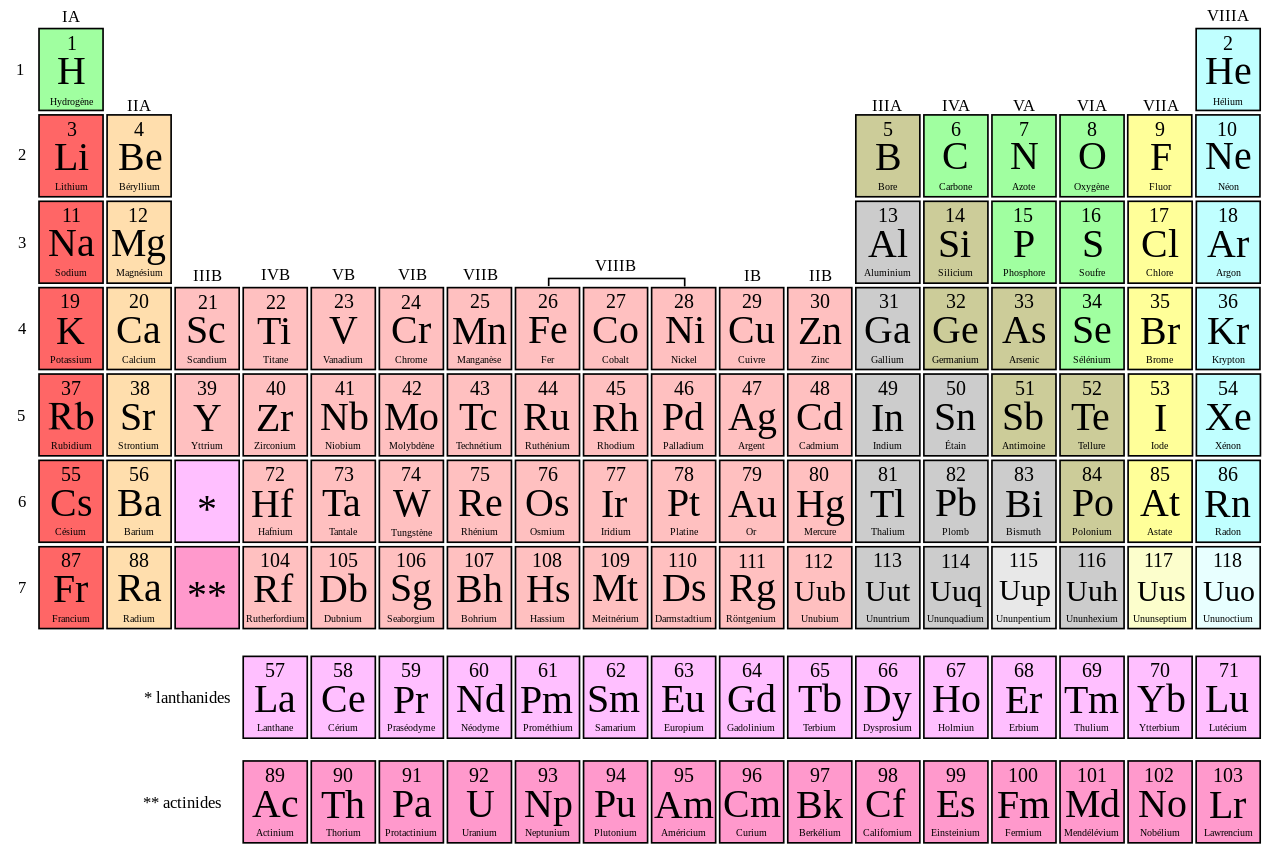
\includegraphics [scale=0.5, angle= 90 ]{img/tableau} 
\ \label{LastPage}

\end{document}